\documentclass[border=2pt]{standalone}
\usepackage[T1]{fontenc}
\usepackage{lmodern}
\usepackage{amsmath,amssymb}
\usepackage{tikz}
\usepackage{pgfplots}
\pgfplotsset{compat=1.17}
\usepgfplotslibrary{groupplots}
\usetikzlibrary{arrows.meta,calc,positioning,fit,backgrounds}

\begin{document}
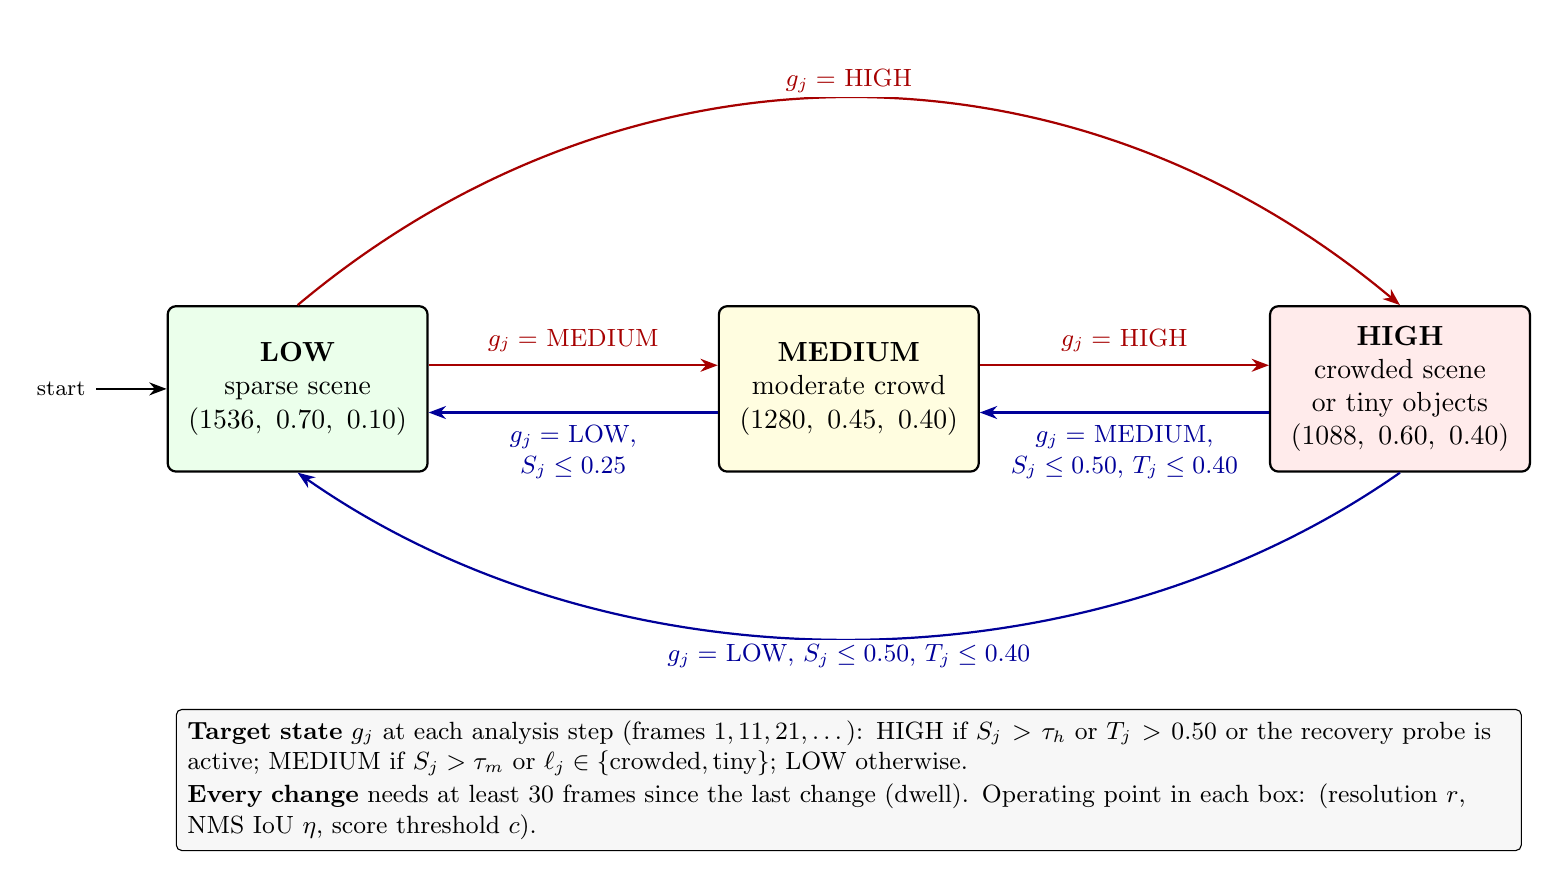
\begin{tikzpicture}[
  font=\normalsize,
  st/.style={draw, rounded corners=3pt, align=center, minimum width=33mm, minimum height=21mm, inner sep=3pt, thick},
  up/.style={-{Stealth[length=2.2mm]}, thick, red!65!black},
  down/.style={-{Stealth[length=2.2mm]}, thick, blue!60!black},
  lab/.style={font=\small, align=center, fill=white, inner sep=1.5pt},
  note/.style={draw, rounded corners=2pt, align=left, font=\small, fill=gray!6, inner sep=4pt, text width=168mm}]
\node[st, fill=green!8]  (low)  at (0,0)    {\textbf{LOW}\\ sparse scene\\ $(1536,\ 0.70,\ 0.10)$};
\node[st, fill=yellow!12] (med) at (7.0,0)  {\textbf{MEDIUM}\\ moderate crowd\\ $(1280,\ 0.45,\ 0.40)$};
\node[st, fill=red!8]    (high) at (14.0,0) {\textbf{HIGH}\\ crowded scene\\ or tiny objects\\ $(1088,\ 0.60,\ 0.40)$};
\draw[{Stealth[length=2.2mm]}-, thick] (low.west) -- ++(-9mm,0) node[left, font=\footnotesize] {start};
% upward changes
\draw[up] ([yshift=3mm]low.east) -- node[lab, above=1mm] {$g_j=$ MEDIUM} ([yshift=3mm]med.west);
\draw[up] ([yshift=3mm]med.east) -- node[lab, above=1mm] {$g_j=$ HIGH} ([yshift=3mm]high.west);
\draw[up] (low.north) to[out=40, in=140] node[lab, above] {$g_j=$ HIGH} (high.north);
% downward changes
\draw[down] ([yshift=-3mm]med.west) -- node[lab, below=1mm] {$g_j=$ LOW,\\ $S_j\le0.25$} ([yshift=-3mm]low.east);
\draw[down] ([yshift=-3mm]high.west) -- node[lab, below=1mm] {$g_j=$ MEDIUM,\\ $S_j\le0.50$, $T_j\le0.40$} ([yshift=-3mm]med.east);
\draw[down] (high.south) to[out=-145, in=-35, looseness=0.9] node[lab, below] {$g_j=$ LOW, $S_j\le0.50$, $T_j\le0.40$} (low.south);
\node[note, below=30mm of med] (n) {%
\textbf{Target state} $g_j$ at each analysis step (frames $1, 11, 21, \dots$):
HIGH if $S_j>\tau_h$ or $T_j>0.50$ or the recovery probe is active;
MEDIUM if $S_j>\tau_m$ or $\ell_j\in\{\text{crowded},\text{tiny}\}$; LOW otherwise.\\[1pt]
\textbf{Every change} needs at least 30 frames since the last change (dwell).
Operating point in each box: (resolution $r$, NMS IoU $\eta$, score threshold $c$).};
\end{tikzpicture}
\end{document}
